\section{Implementation} \label{sec:implementation}
We are now interested in how the theory that we have presented is implemented in simulation programs. DFT is widely used for simulating many systems, from atoms to crystals. However, it is mainly employed to study solid state systems. The main reason is that in crystals, we can take advantage of the symmetries of the system to simplify the computation. We have shown in \cref{sec:crystals} that crystals are periodic systems, were the periodicity is governed by the lattice vectors $\vec{R}_n$. Every property, included the ion potential, shares the same periodicity. The central consequence is that the solutions to the \sche for this kind of potential can be written in a Block form
\begin{equation}
    \Psi_{\vec{k}}(\vec{r}) = u_{\vec{k}}(\vec{r}) e^{i\vec{k}\cdot\vec{r}}
\end{equation}
where $\vec{k}$ is the wavevector and $u_{\vec{k}}(\vec{r})$ is a function with the same periodicity of the lattice, that is $u_{\vec{k}}(\vec{r}) = u_{\vec{k}}(\vec{r}+\vec{R}_n)$. We can use this fact to expand $u_{\vec{k}}(\vec{r})$ in a Fourier series
\begin{equation}
    u_{\vec{k}}(\vec{r}) = \sum_\vec{G} c_{\vec{k}+\vec{G}} e^{i\vec{G}\cdot\vec{r}}
\end{equation}
where $\vec{G}$ are reciprocal lattice vectors and $c_{\vec{k}+\vec{G}}$ are constants. The general solution of the \sche is then
\begin{equation} \label{eq:sum_bloch}
    \Psi_{\vec{k}}(\vec{r}) = \sum_\vec{G} c_{\vec{k}+\vec{G}} e^{i(\vec{k}+\vec{G})\cdot\vec{r}}
\end{equation}

Wavefunctions in the Bloch form are not only easier to manage, but they offer significant advantages in performing computations. In fact, solving \cref{eq:kohn_sche} requires solving many integrals of the form $\bra{\Psi_{\vec{k}}(\vec{r})} \oper{H} \ket{\Psi_{\vec{k}}(\vec{r})}$. For a given value of $\vec{k}$, the integrals should be performed over the whole space. This would be very computationally demanding. Fortunately, if $\Psi_{\vec{k}}(\vec{r})$ is a Bloch function, it can be proven that the solution of the integral are given by the sum of the band energies $\epsilon_n$, so
\begin{equation}
    \bra{\Psi_{\vec{k}}(\vec{r})} \oper{H} \ket{\Psi_{\vec{k}}(\vec{r})} = \frac{\Omega}{(2\pi)^3} \sum_n \int_\text{BZ} \epsilon_n(\vec{k})\differential \vec{k}
\end{equation}
where $\Omega$ is the volume of the unit cell and the integral is extended over the fist Brillouin zone. This integral is much easier to compute. In practical calculations, the integral over the Brillouin zone is evaluated only on a finite set of points. The most common choice for this set of points is the Monkhorst-Pack grid \cite{monkhorst1976}. In fractional coordinates, it is a rectangular grid spaced evenly throughout the Brillouin zone. The main advantage of this method is that it gives accurate results even with a small number of points.

Sometimes, the integration has problems to converge because of the discontinuity points of the function. This is particularly common in metals, where it is common to have regions in the reciprocal space where the electronic density suddenly drops to zero. To avoid this inconvenience, the discontinuity regions are softened applying \emph{smearing} functions. For example, it is common to use gaussian functions centered in the discontinuity and parametrized by their standard deviation $\sigma$. In the limit $\sigma \rightarrow 0$ there is no smearing, and the discontinuity is not eliminated.

The problem of solving the Kohn-Sham equations is not completely solved yet. In fact, in \cref{eq:sum_bloch} the sum is extended over an infinite number of reciprocal lattice vectors $\vec{G}$, so it is not possible to evaluate it exactly. Luckily, the single terms in the sum may be interpreted as solutions to \sches with a corresponding kinetic energy
\begin{equation}
    E_\vec{k} = \frac{\hslash^2(\vec{k}+\vec{G})^2}{2m}
\end{equation}
The higher energy terms will have less physical meaning, so they can be excluded from the sum. This is done by choosing a cutoff value $E_\text{cut}$ and a corresponding value $G_\text{cut}$, and ignoring the terms with $|\vec{G}| < G_\text{cut}$.

Usually, in DFT applications, another simplification is made. Since most of the properties of materials are determined only by the valence electrons, the ion-electron interaction is determined using pseudopotentials. With pseudopotentials, the core electrons are removed from the calculation, and they are replaced with an effective potential. Only the valence electrons (or the valence and outer core electrons) are simulated. In addition to reducing the number of electrons that have to be simulated, pseudopotentials offer a second advantage. The valence electrons wavefunctions oscillate rapidly near the nucleus because of the strong nuclear potential, as it can be seen in \cref{fig:pseudopotential}. The rapid oscillations in the region close to the nucleus require high frequency cutoff energies for the plane waves, impacting on the simulation performance. Pseudopotentials "smoothen" the wavefunctions, allowing to choose a smaller $G_\text{cut}$ and making the computation faster.

\begin{figure}
    \centering
    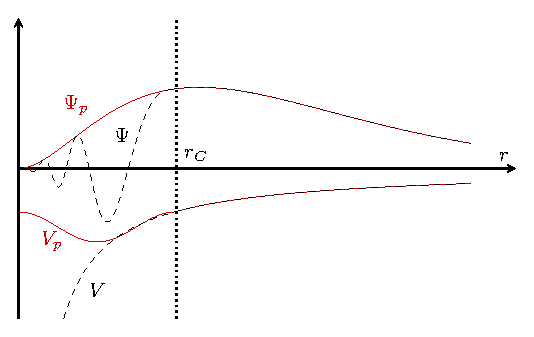
\includegraphics[width=0.5\textwidth]{figures/pseudopotential/pseudopotential.pdf}
    \caption[Pseudopotentials]{Comparison of a wavefunction in the Coulomb potential of the nucleus (black line) and in a pseudopotential (red line). The wavefunctions and potentials coincide for distances greater than $r_C$.}
    \label{fig:pseudopotential}
\end{figure}
